\documentclass[tikz,border=2pt]{standalone}
\renewcommand{\familydefault}{\sfdefault}
\usetikzlibrary{arrows.meta,calc,positioning}
\tikzset{every picture/.style={line width=1pt, >=Stealth},
         hl/.style={fill=black, fill opacity=0.12, text opacity=1}}
\begin{document}
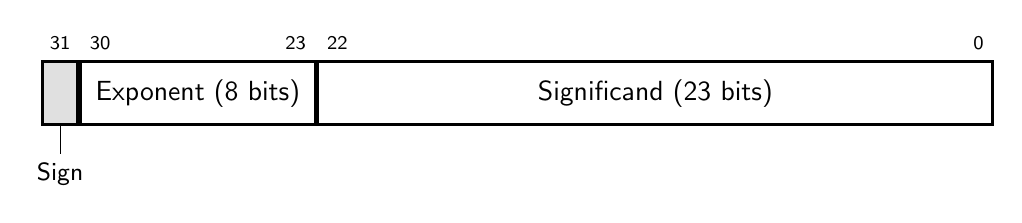
\begin{tikzpicture}[field/.style={draw, minimum height=0.8cm, anchor=west}, bit/.style={font=\scriptsize, above}]
  % Field widths are proportional to their bit counts (the sign is widened to stay visible).
  \node[field, hl, minimum width=0.45cm] (sign) at (0, 0) {};
  \node[field, minimum width=2.98cm] (exp) at (sign.east) {Exponent (8 bits)};
  \node[field, minimum width=8.57cm] (sig) at (exp.east) {Significand (23 bits)};
  \draw[thin] (sign.south) -- ++(0, -0.35) node[below, font=\small] {Sign};
  % Bit indices, most significant on the left
  \node[bit] at (sign.north) {31};
  \node[bit, anchor=south west] at (exp.north west) {30};
  \node[bit, anchor=south east] at (exp.north east) {23};
  \node[bit, anchor=south west] at (sig.north west) {22};
  \node[bit, anchor=south east] at (sig.north east) {0};
\end{tikzpicture}
\end{document}
